\documentclass[a4paper,10pt]{article}

\usepackage{sig33,graphicx}
\usepackage{hyperref}

% usepackage for url
\usepackage{url}

\begin{document}
%
% Please underline the presenting author and give
% at least the email address of that author.
%

\title{Influence of Mach Number and 3D Instabilities on the Transition Mechanisms of Laminar Boundary Layers over Gap Discontinuities}

\author{\underline{Víctor Ballester Ribó}$^1$, Jeffrey Crouch$^2$, Yongyun Hwang$^1$, Spencer Sherwin$^1$}
\affiliation{$^1$Department of Aeronautics, Imperial College London, UK \ $^2$The Boeing Company, USA}

\maketitle

In this work we investigate the linear stability of laminar boundary layers encountering a gap discontinuity. The gap is modeled as a rectangular cavity of width $w$ and depth $d$ embedded in a flat plate aligned with the flow. The depth of the cavity is varied within the range $d/\delta^* \in [0.5, 4]$, while the width is set to $w/\delta^* \in [5, 100]$. The Reynolds number considered is $\textrm{Re}_{\delta^*} = 1000$, where $\delta^*$ denotes the displacement thickness measured at the upstream edge of the gap on a smooth surface that is free of discontinuities. High-fidelity simulations for both incompressible and compressible flows are performed using the spectral/\emph{hp} element method implemented in Nektar++~\cite{nektarpp}. Under incompressible or low-Mach-number conditions, previous experimental studies~\cite{jeffGaps} have shown that narrow gaps amplify Tollmien--Schlichting (TS) waves, leading to transition downstream through the primary instability pathway, as illustrated in Figure~\ref{fig:tstrans}. In contrast, sufficiently wide gaps promote a bypass transition originating near the downstream edge of the gap. In incompressible simulations, for fixed gap depth $d$, a Hopf bifurcation emerges as the gap width exceeds a critical value $\mathcal{H}(d)$. The periodic orbit emerges as a form of self-sustained oscillation near the downstream edge of the gap. The critical width for this bifurcation increases as the gap depth decreases and disappears for shallow gaps ($d/\delta^* < 1.25$), which remain globally stable. The functions $d\mapsto \mathcal{B}(d)$ (bypass threshold) and $d\mapsto \mathcal{H}(d)$ show good agreement. We further extend the analysis to examine the effects of Mach number ($\textrm{M} \in (0,1)$) and three-dimensional gap geometries on the bifurcation behavior. Results indicate that increasing Mach number lowers the critical width $\mathcal{H}(d)$, suggesting that compressibility promotes bypass transition.

\begin{figure}[!ht]
	\centering
	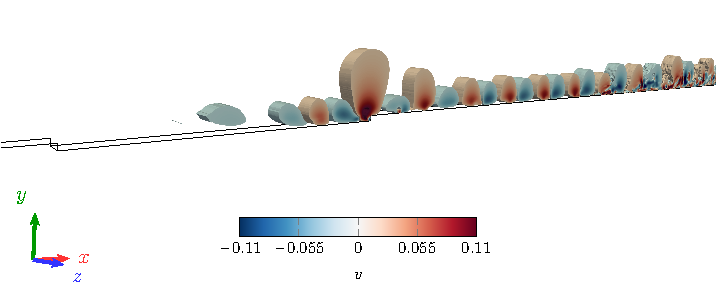
\includegraphics[width=\linewidth]{../../Images/tstransition_d1.5w80.pdf}
	\vspace{-0.5cm}
	\caption{Wall-normal velocity isovolumes showing the over-amplification of TS waves due to the presence of a 3D gap discontinuity of depth $d = 1.5 \delta^*$ and width $w = 80\delta^*$, and transition to turbulence downstream of the gap.}
	\label{fig:tstrans}
\end{figure}

\begin{thebibliography}{1}

  \bibitem{nektarpp}
  C.~D. Cantwell, S.~J. Sherwin, R.~M. Kirby, and P.~H. J. Kelly.
  \newblock{Nektar++: An open-source spectral/\(hp\) element framework.}
  \newblock{{\em Comput. Phys. Commun.}, 192:205--219, 2015.}
  \newblock{DOI: \url{10.1016/j.cpc.2015.02.008}.}

	\bibitem{jeffGaps}
	J.~D. Crouch, V.~S. Kosorygin, M.~I. Sutanto, and G.~D. Miller.
	\newblock{Characterizing surface-gap effects on boundary-layer transition dominated by Tollmien--Schlichting instability.}
	\newblock{\em Flow}, 2:E8, 2022.
	\newblock{DOI: \url{10.1017/flo.2022.1}.}

\end{thebibliography}

\end{document}
